%% 
%% Copyright 2019-2020 Elsevier Ltd
%% 
%% This file is part of the 'CAS Bundle'.
%% --------------------------------------
%% 
%% It may be distributed under the conditions of the LaTeX Project Public
%% License, either version 1.2 of this license or (at your option) any
%% later version.  The latest version of this license is in
%%    http://www.latex-project.org/lppl.txt
%% and version 1.2 or later is part of all distributions of LaTeX
%% version 1999/12/01 or later.
%% 
%% The list of all files belonging to the 'CAS Bundle' is
%% given in the file `manifest.txt'.
%% 
%% Template article for cas-sc documentclass for 
%% double column output.

%\documentclass[a4paper,fleqn,longmktitle]{cas-sc}
\documentclass[a4paper,fleqn]{cas-sc}

% \usepackage[numbers]{natbib}
%\usepackage[authoryear]{natbib}
\usepackage[authoryear,longnamesfirst]{natbib}

%%%Author definitions
\def\tsc#1{\csdef{#1}{\textsc{\lowercase{#1}}\xspace}}
\tsc{WGM}
\tsc{QE}
\tsc{EP}
\tsc{PMS}
\tsc{BEC}
\tsc{DE}
%%%

% Uncomment and use as if needed
%\newtheorem{theorem}{Theorem}
%\newtheorem{lemma}[theorem]{Lemma}
%\newdefinition{rmk}{Remark}
%\newproof{pf}{Proof}
%\newproof{pot}{Proof of Theorem \ref{thm}}

\begin{document}
\let\WriteBookmarks\relax
\def\floatpagepagefraction{1}
\def\textpagefraction{.001}

% Short title
\shorttitle{Leveraging social media news}

% Short author
\shortauthors{CV Radhakrishnan et~al.}

% Main title of the paper
\title [mode = title]{Let Me Tell You The Facts: }                      
% Title footnote mark
% eg: \tnotemark[1]
\tnotemark[1,2]

% Title footnote 1.
% eg: \tnotetext[1]{Title footnote text}
% \tnotetext[<tnote number>]{<tnote text>} 

% First author
%
% Options: Use if required
% eg: \author[1,3]{Author Name}[type=editor,
%       style=chinese,
%       auid=000,
%       bioid=1,
%       prefix=Sir,
%       orcid=0000-0000-0000-0000,
%       facebook=<facebook id>,
%       twitter=<twitter id>,
%       linkedin=<linkedin id>,
%       gplus=<gplus id>]
\author[1,3]{CV Radhakrishnan}[type=editor,
                        auid=000,bioid=1,
                        prefix=Sir,
                        role=Researcher,
                        orcid=0000-0001-7511-2910]

% Corresponding author indication
\cormark[1]

% Footnote of the first author
\fnmark[1]

% Email id of the first author
\ead{cvr_1@tug.org.in}

% URL of the first author
\ead[url]{www.cvr.cc, cvr@sayahna.org}

%  Credit authorship
%\credit{Conceptualization of this study, Methodology, Software}

% Address/affiliation
\affiliation[1]{organization={Elsevier B.V.},
    addressline={Radarweg 29}, 
    city={Amsterdam},
    % citysep={}, % Uncomment if no comma needed between city and postcode
    postcode={1043 NX}, 
    % state={},
    country={The Netherlands}}

% Second author
\author[2,4]{Han Theh Thanh}[style=chinese]

% Third author
\author[2,3]{CV Rajagopal}[%
   role=Co-ordinator,
   suffix=Jr,
   ]
\fnmark[2]
\ead{cvr3@sayahna.org}
\ead[URL]{www.sayahna.org}

%\credit{Data curation, Writing - Original draft preparation}

% Address/affiliation
\affiliation[2]{organization={Sayahna Foundation},
    % addressline={}, 
    city={Jagathy},
    % citysep={}, % Uncomment if no comma needed between city and postcode
    postcode={695014}, 
    state={Trivandrum},
    country={India}}

% Fourth author
\author%
[1,3]
{Rishi T.}
\cormark[2]
\fnmark[1,3]
\ead{rishi@stmdocs.in}
\ead[URL]{www.stmdocs.in}

\affiliation[3]{organization={STM Document Engineering Pvt Ltd.},
    addressline={Mepukada}, 
    city={Malayinkil},
    % citysep={}, % Uncomment if no comma needed between city and postcode
    postcode={695571}, 
    state={Trivandrum},
    country={India}}

% Corresponding author text
%\cortext[cor1]{Corresponding author}
%\cortext[cor2]{Principal corresponding author}

% Footnote text

% For a title note without a number/mark


% Here goes the abstract
\begin{abstract}
This template helps you to create a properly formatted \LaTeX\ manuscript.
\noindent\texttt{\textbackslash begin{abstract}} \dots 
\texttt{\textbackslash end{abstract}} and
\verb+\begin{keyword}+ \verb+...+ \verb+\end{keyword}+ 
which
contain the abstract and keywords respectively. 

\noindent Each keyword shall be separated by a \verb+\sep+ command.
\end{abstract}

% Use if graphical abstract is present
% \begin{graphicalabstract}
% \includegraphics{figs/grabs.pdf}
% \end{graphicalabstract}

% Research highlights
\begin{highlights}
\item Research highlights item 1111
\item Research highlights item 2
\item Research highlights item 3
\end{highlights}

% Keywords
% Each keyword is seperated by \sep
\begin{keywords}
quadrupole exciton \sep polariton \sep \WGM \sep \BEC
\end{keywords}

\maketitle


\section{Results}
In this study, we conducted an empirical investigation to evaluate the impact of interaction types(web v.s. chatbot) and correction formats(highlighting expert titles or not) on fact-checking effectiveness(RQ1), cognitive effort(RQ2) and further analyzed which conditions help increase users' intention to use. 
For ease of description, we use \textbf{Interaction*Format} to denote our experimental conditions. 
"Interaction" can be classified as "web" and "chatbot", which refer to using the webpage or the chatbot to obtain fact-checking results, respectively.  
"Format" can be "Regular" or "Highlighted"(Highlighted expert titles).

We used the two-way ANOVA to examine the main effects and interactions.
Before that, a Shapiro-Wilk normality test was conducted to validate the normality assumption. The results showed that our data violated this assumption. 
Therefore, we used the Aligned Rank Transform(ART) procedure from the R-language Artool package to conduct the nonparametric factorial ANOVA.

\begin{table}[width=.9\linewidth,cols=5,pos=h]
    \caption{Descriptive Analysis of all measured dependent validate}\label{tbl1}
    \label{tab:descriptive}
    \begin{tabular*}{\tblwidth}{@{} LCCCC@{} }
    \toprule
    \textbf{Dependent}&\textbf{Web*Regualr}&\textbf{Web*Expert}&\textbf{Chatbot*Regualr} & \textbf{Chatbot*Expert}\\
    \textbf{variable}&(N=74)&(N=72)&(N=78)&(N=84)\\
     & Mean (SD) & Mean (SD) & Mean (SD) & Mean (SD) \\
    \midrule
    \textbf{Perceived Effectiveness}&\textbf{4.29 (0.63)} & 4.04 (0.75) & 4.11(0.73) & 4.28(0.58)\\
    \textbf{Actual Effectiveness}&1.51 (1.47) & 1.57 (1.47) & 1.79(1.22) & \textbf{1.82(1.44)}\\
    \textbf{Cognitive Effort}&3.86 (0.73) & 3.68 (0.76) & 4.15(0.67) & \textbf{4.17(0.74)}\\
    \textbf{Intention to Use}&3.98 (0.86) & 3.69 (0.82) & 3.93(0.68) & \textbf{4.00(0.67)}\\
    \bottomrule
    \end{tabular*}
    \end{table} 

    \begin{figure*}
        \centering
          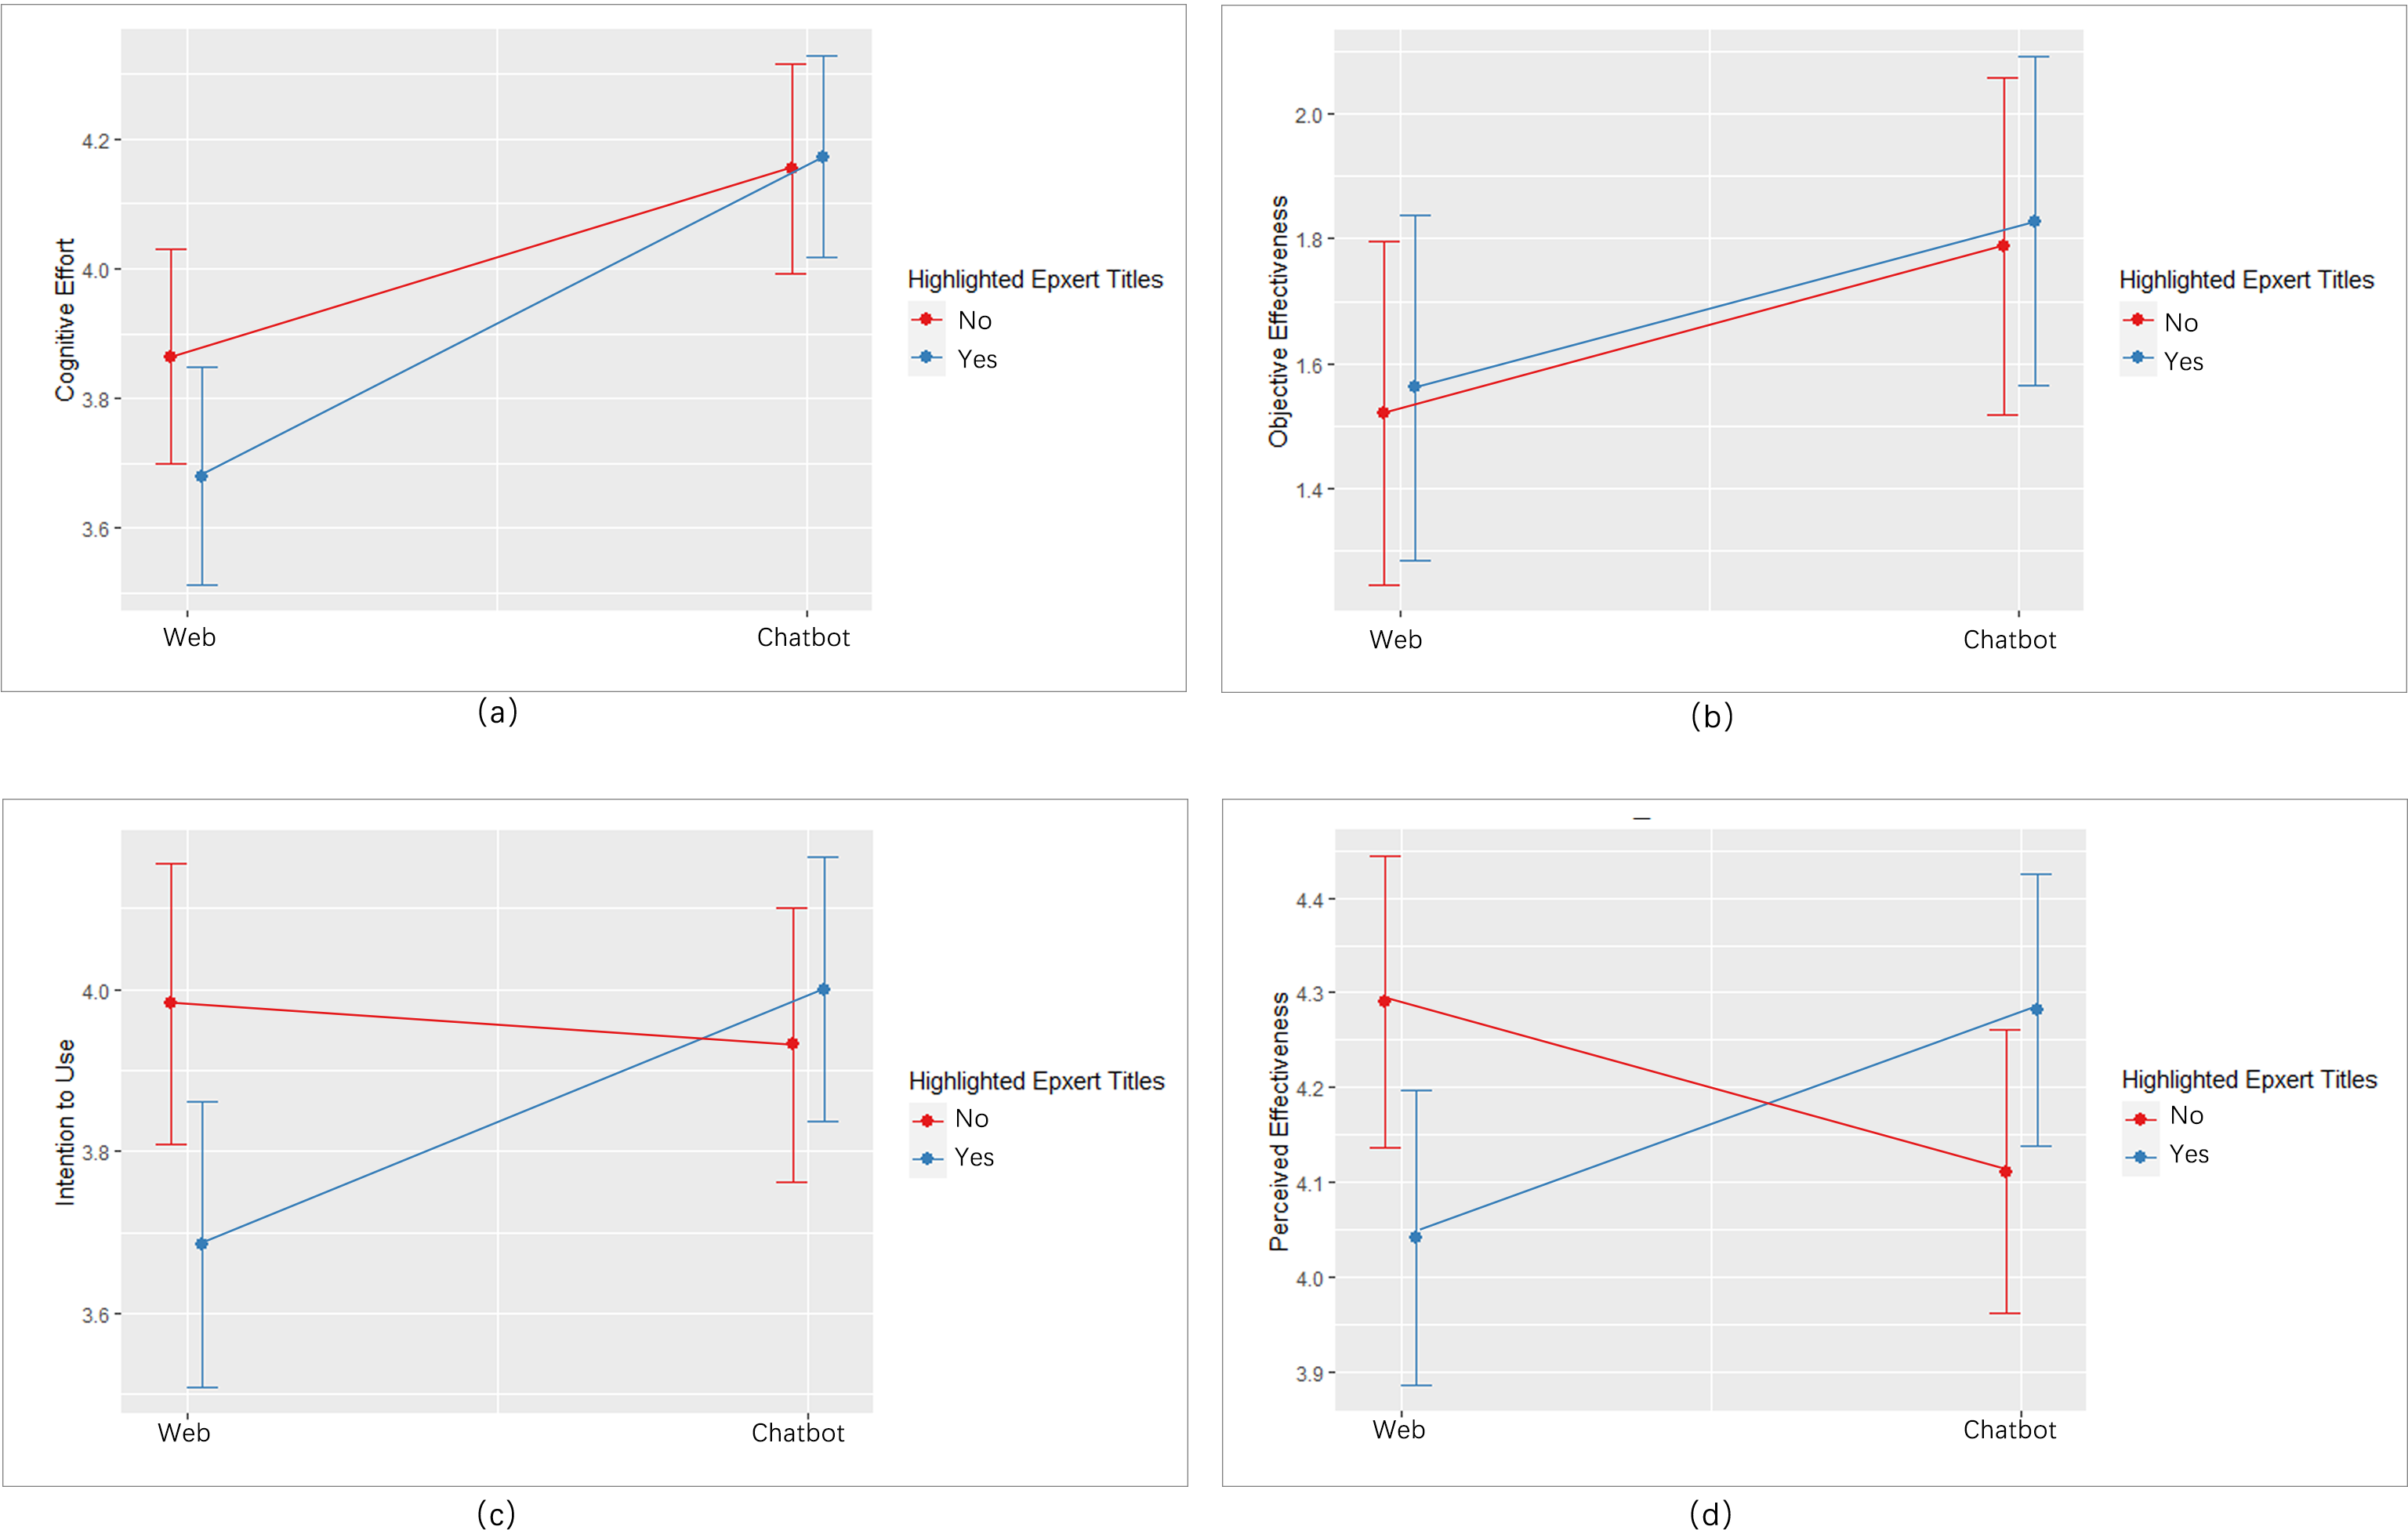
\includegraphics[width=\textwidth,height=4.6in]{figs/fig_main_interaction.png}
        \caption{The results of nonparametric factorial ANOVA.The interaction type has a significant main effect on (a) cognitive effects and a weak main effect on (b) objective effectiveness. 
        The chatbot is more likely to reduce users' cognitive effort and improve the actual effectiveness of correction.
        Two significant intention effects exist between interaction type and currection format on (c) perceived effectiveness and (d) intention to use.}
        \label{FIG:interaction}
    \end{figure*}

\subsection{Evaluation of Currection Effectiveness}
To comprehensively measure the correction effectiveness, we evaluated the experimental conditions from both subjective and objective aspects.
The results revealed an interaction effect in subjective effectiveness, while there was no significant difference in actual effectiveness.

\subsubsection{Perceived Effectiveness}
The 2*2 ANOVA shows a significant interaction effect between interaction type and format on perceived effectiveness, F(1, 323)=6.31, p<0.05, $\eta^{2}$=0.020.
We can observe that when participants use the web for fact-checking, the emphasis on expert titles decreases their perceived effectiveness.
However, there is an opposite trend when using the chatbot(see Figure~\ref{FIG:interaction}(d)).
Besides, the Chatbot*Highlighted design has a similar level of perceived effectiveness with the Web*Regualr(Table~\ref{tab:descriptive}).

\subsubsection{ Objectiveness Effectiveness}

Table~\ref{tab:descriptive} shows the participants' performance on the objective effectiveness questions. 
Participants answered the same questions in both tests, and we measured objective effectiveness by the increased number of correct answers to objective questions.
It can be seen that participants had better performance in the chatbot condition, while there was no significant effect on whether or not the expert title was highlighted.
In the web condition, participants' correct responses increased by 1.51 and 1.57 in the "Regular" and the "Highlighted" conditions, while in the chatbot condition, the increases were 1.79 and 1.82, respectively.
The results of two-way ANOVA show a weak significant main effect on the interaction type.

\subsection{Evaluation of Users' Intention}
We examine the impact of the tool on user's behavioral tendencies from both their intention to use this tool and their intention to fact-check it in the future.
Before that we measured the cognitive effort of users in different experimental conditions.
As mentioned before, people are not willing to spend extra cognitive effort to verify the authenticity of information. If the design can help users reduce the cognitive effort, this may have a positive impact on their behavioral tendencies, which is the reason we measured this variable.
There, higher values of the variable indicate easier of use and less cognitive effort.

\subsubsection{Cognitive Effort}
Analysis of cognitive effort yields a significant main effect of interaction type, F(1, 323)=20.239, p < 0.001, $\eta^{2}$ = 0.059, indicating that participants expend less cognitive effort to check facts when using chatbots compared to using the web(see Figure~\ref{FIG:interaction}(a)). 
The results do not show a significant main effect of format or an interaction effect.

\subsubsection{Intention to Use}
The main effects of interaction type and format are not found, but the interaction effect is significant, F (1, 323) = 5.310, p < 0.05, $\eta^{2}$ =0.022. 
Participants in the highlighted format reported lower intention to use than in the normal format condition when they use the web, but this effect disappears under the chatbot condition(see Figure~\ref{FIG:interaction}(b)).
There is no significant difference between the regular and highlighted formats when the chatbot is applied. Besides, the chatbot*highlighted design leads to the highest intention to use(Mean=3.993,SD=0.680).



\printcredits

%% Loading bibliography style file
% \bibliographystyle{model1-num-names}
\bibliographystyle{cas-model2-names}

% Loading bibliography database
\bibliography{cas-refs}


%\vskip3pt


\end{document}

